% ============================================================
% Question Bank: ch05-04 Solving Multi-Step Problems with Rational Numbers
% Topic Title: Solving Multi-Step Problems with Rational Numbers
% CCSS: 7.EE.B.3
% Questions: 27 (15 MC + 6 SA + 6 Graphical)
% ============================================================

% --- Multiple Choice Questions (15) ---

\begin{practiceQuestion}{5-4-q01}{mc}
\begin{questionText}
Solve $0.4x + 3.2 = 7.2$.
\end{questionText}
\choiceA{$x = 10$}
\choiceB{$x = 26$}
\choiceC{$x = 1$}
\choiceD{$x = 16$}
\correctAnswer{A}
\explanation{Subtract $3.2$: $0.4x = 4$. Divide by $0.4$: $x = 10$. Check: $0.4(10) + 3.2 = 4 + 3.2 = 7.2$ \checkmark.}
\end{practiceQuestion}

\begin{practiceQuestion}{5-4-q02}{mc}
\begin{questionText}
Solve $\dfrac{x}{5} + \dfrac{2}{5} = 3$.
\end{questionText}
\choiceA{$x = 13$}
\choiceB{$x = 15$}
\choiceC{$x = 17$}
\choiceD{$x = 1$}
\correctAnswer{A}
\explanation{Multiply every term by $5$: $x + 2 = 15$. Subtract $2$: $x = 13$. Check: $\frac{13}{5} + \frac{2}{5} = \frac{15}{5} = 3$ \checkmark.}
\end{practiceQuestion}

\begin{practiceQuestion}{5-4-q03}{mc}
\begin{questionText}
Solve $-0.5y + 6 = 2$.
\end{questionText}
\choiceA{$y = -8$}
\choiceB{$y = 8$}
\choiceC{$y = 16$}
\choiceD{$y = -16$}
\correctAnswer{B}
\explanation{Subtract $6$: $-0.5y = -4$. Divide by $-0.5$: $y = 8$. Check: $-0.5(8) + 6 = -4 + 6 = 2$ \checkmark.}
\end{practiceQuestion}

\begin{practiceQuestion}{5-4-q04}{mc}
\begin{questionText}
Which is the best first step to solve $\dfrac{x}{3} + \dfrac{1}{6} = 2$?
\end{questionText}
\choiceA{Subtract $\frac{1}{6}$ from both sides}
\choiceB{Multiply every term by $6$}
\choiceC{Divide both sides by $3$}
\choiceD{Add $\frac{1}{6}$ to both sides}
\correctAnswer{B}
\explanation{Multiplying every term by $6$ (the LCD) clears the fractions: $2x + 1 = 12$.}
\end{practiceQuestion}

\begin{practiceQuestion}{5-4-q05}{mc}
\begin{questionText}
Solve $\dfrac{3x}{4} + 2 = 11$.
\end{questionText}
\choiceA{$x = 12$}
\choiceB{$x = 6$}
\choiceC{$x = 36$}
\choiceD{$x = 17\frac{1}{3}$}
\correctAnswer{A}
\explanation{Subtract $2$: $\frac{3x}{4} = 9$. Multiply by $4$: $3x = 36$. Divide by $3$: $x = 12$. Check: $\frac{3(12)}{4} + 2 = 9 + 2 = 11$ \checkmark.}
\end{practiceQuestion}

\begin{practiceQuestion}{5-4-q06}{mc}
\begin{questionText}
Solve $1.5n - 4.5 = 6$.
\end{questionText}
\choiceA{$n = 1$}
\choiceB{$n = 3$}
\choiceC{$n = 7$}
\choiceD{$n = 10.5$}
\correctAnswer{C}
\explanation{Add $4.5$: $1.5n = 10.5$. Divide by $1.5$: $n = 7$. Check: $1.5(7) - 4.5 = 10.5 - 4.5 = 6$ \checkmark.}
\end{practiceQuestion}

\begin{practiceQuestion}{5-4-q07}{mc}
\begin{questionText}
A recipe uses $\dfrac{2}{3}$ cup of flour per batch of muffins. You used $\dfrac{1}{3}$ cup testing and have $3$ cups total. The equation $\dfrac{2}{3}b + \dfrac{1}{3} = 3$ finds how many batches $b$ you can make. What is $b$?
\end{questionText}
\choiceA{$b = 4$}
\choiceB{$b = 3$}
\choiceC{$b = 5$}
\choiceD{$b = 2$}
\correctAnswer{A}
\explanation{Subtract $\frac{1}{3}$: $\frac{2}{3}b = \frac{8}{3}$. Multiply by $\frac{3}{2}$: $b = \frac{8}{3} \times \frac{3}{2} = 4$.}
\end{practiceQuestion}

\begin{practiceQuestion}{5-4-q08}{mc}
\begin{questionText}
Solve $\dfrac{x}{6} - \dfrac{1}{3} = \dfrac{3}{2}$.
\end{questionText}
\choiceA{$x = 11$}
\choiceB{$x = 7$}
\choiceC{$x = 8$}
\choiceD{$x = 12$}
\correctAnswer{A}
\explanation{Multiply every term by $6$: $x - 2 = 9$. Add $2$: $x = 11$. Check: $\frac{11}{6} - \frac{1}{3} = \frac{11}{6} - \frac{2}{6} = \frac{9}{6} = \frac{3}{2}$ \checkmark.}
\end{practiceQuestion}

\begin{practiceQuestion}{5-4-q09}{mc}
\begin{questionText}
Solve $2.5x + 1.5 = 11.5$.
\end{questionText}
\choiceA{$x = 4$}
\choiceB{$x = 5.2$}
\choiceC{$x = 5$}
\choiceD{$x = 2.6$}
\correctAnswer{A}
\explanation{Subtract $1.5$: $2.5x = 10$. Divide by $2.5$: $x = 4$. Check: $2.5(4) + 1.5 = 10 + 1.5 = 11.5$ \checkmark.}
\end{practiceQuestion}

\begin{practiceQuestion}{5-4-q10}{mc}
\begin{questionText}
A student estimates that the solution to $0.35x + 2.8 = 9.8$ is about $x = 20$. Is this estimate reasonable?
\end{questionText}
\choiceA{Yes, the exact answer is $20$}
\choiceB{Yes, the exact answer is close to $20$}
\choiceC{No, the exact answer is about $37$}
\choiceD{No, the exact answer is about $10$}
\correctAnswer{A}
\explanation{Subtract $2.8$: $0.35x = 7$. Divide by $0.35$: $x = 20$. The estimate is exactly correct.}
\end{practiceQuestion}

\begin{practiceQuestion}{5-4-q11}{mc}
\begin{questionText}
Solve $-2.4x + 3.6 = -1.2$.
\end{questionText}
\choiceA{$x = -2$}
\choiceB{$x = 1$}
\choiceC{$x = 2$}
\choiceD{$x = -1$}
\correctAnswer{C}
\explanation{Subtract $3.6$: $-2.4x = -4.8$. Divide by $-2.4$: $x = 2$. Check: $-2.4(2) + 3.6 = -4.8 + 3.6 = -1.2$ \checkmark.}
\end{practiceQuestion}

\begin{practiceQuestion}{5-4-q12}{mc}
\begin{questionText}
Solve $\dfrac{n}{3} + \dfrac{n}{6} = 5$.
\end{questionText}
\choiceA{$n = 10$}
\choiceB{$n = 15$}
\choiceC{$n = 6$}
\choiceD{$n = 30$}
\correctAnswer{A}
\explanation{Multiply every term by $6$: $2n + n = 30$. Combine: $3n = 30$. Divide by $3$: $n = 10$. Check: $\frac{10}{3} + \frac{10}{6} = \frac{20}{6} + \frac{10}{6} = \frac{30}{6} = 5$ \checkmark.}
\end{practiceQuestion}

\begin{practiceQuestion}{5-4-q13}{mc}
\begin{questionText}
A jacket originally costs $p$ dollars. It is discounted by $\dfrac{1}{4}$ of the price, then an additional $\$10$ is taken off. The final price is $\$50$. What equation finds $p$?
\end{questionText}
\choiceA{$\dfrac{1}{4}p - 10 = 50$}
\choiceB{$\dfrac{3}{4}p + 10 = 50$}
\choiceC{$\dfrac{3}{4}p - 10 = 50$}
\choiceD{$p - \dfrac{1}{4} - 10 = 50$}
\correctAnswer{C}
\explanation{After $\frac{1}{4}$ off: $p - \frac{p}{4} = \frac{3p}{4}$. After $\$10$ more off: $\frac{3p}{4} - 10 = 50$.}
\end{practiceQuestion}

\begin{practiceQuestion}{5-4-q14}{mc}
\begin{questionText}
Solve $0.8x - 3.2 = 4.8$.
\end{questionText}
\choiceA{$x = 10$}
\choiceB{$x = 2$}
\choiceC{$x = 1$}
\choiceD{$x = 6.4$}
\correctAnswer{A}
\explanation{Add $3.2$: $0.8x = 8$. Divide by $0.8$: $x = 10$. Check: $0.8(10) - 3.2 = 8 - 3.2 = 4.8$ \checkmark.}
\end{practiceQuestion}

\begin{practiceQuestion}{5-4-q15}{mc}
\begin{questionText}
Solve $\dfrac{5x}{3} - 4 = 6$.
\end{questionText}
\choiceA{$x = 2$}
\choiceB{$x = 6$}
\choiceC{$x = 30$}
\choiceD{$x = 15$}
\correctAnswer{B}
\explanation{Add $4$: $\frac{5x}{3} = 10$. Multiply by $3$: $5x = 30$. Divide by $5$: $x = 6$. Check: $\frac{5(6)}{3} - 4 = 10 - 4 = 6$ \checkmark.}
\end{practiceQuestion}

% --- Short Answer Questions (6) ---

\begin{practiceQuestion}{5-4-q16}{sa}
\begin{questionText}
Solve $\dfrac{2x}{3} + 5 = 11$.
\end{questionText}
\correctAnswer{$x = 9$}
\explanation{Subtract $5$: $\frac{2x}{3} = 6$. Multiply by $3$: $2x = 18$. Divide by $2$: $x = 9$. Check: $\frac{2(9)}{3} + 5 = 6 + 5 = 11$ \checkmark.}
\end{practiceQuestion}

\begin{practiceQuestion}{5-4-q17}{sa}
\begin{questionText}
Solve $0.6y + 1.8 = 6$.
\end{questionText}
\correctAnswer{$y = 7$}
\explanation{Subtract $1.8$: $0.6y = 4.2$. Divide by $0.6$: $y = 7$. Check: $0.6(7) + 1.8 = 4.2 + 1.8 = 6$ \checkmark.}
\end{practiceQuestion}

\begin{practiceQuestion}{5-4-q18}{sa}
\begin{questionText}
Solve $\dfrac{x}{4} + \dfrac{1}{2} = \dfrac{7}{4}$.
\end{questionText}
\correctAnswer{$x = 5$}
\explanation{Multiply every term by $4$: $x + 2 = 7$. Subtract $2$: $x = 5$. Check: $\frac{5}{4} + \frac{1}{2} = \frac{5}{4} + \frac{2}{4} = \frac{7}{4}$ \checkmark.}
\end{practiceQuestion}

\begin{practiceQuestion}{5-4-q19}{sa}
\begin{questionText}
Solve $-0.25n + 3 = 1$.
\end{questionText}
\correctAnswer{$n = 8$}
\explanation{Subtract $3$: $-0.25n = -2$. Divide by $-0.25$: $n = 8$. Check: $-0.25(8) + 3 = -2 + 3 = 1$ \checkmark.}
\end{practiceQuestion}

\begin{practiceQuestion}{5-4-q20}{sa}
\begin{questionText}
A store reduces a pair of shoes by $\dfrac{1}{5}$ of the original price $p$, then gives a $\$6$ loyalty discount. The final price is $\$42$. Find the original price.
\end{questionText}
\correctAnswer{$p = \$60$}
\explanation{After $\frac{1}{5}$ off: $p - \frac{p}{5} = \frac{4p}{5}$. After $\$6$ off: $\frac{4p}{5} - 6 = 42$. Add $6$: $\frac{4p}{5} = 48$. Multiply by $\frac{5}{4}$: $p = 60$.}
\end{practiceQuestion}

\begin{practiceQuestion}{5-4-q21}{sa}
\begin{questionText}
Solve $\dfrac{7n}{4} + \dfrac{3}{2} = 5$.
\end{questionText}
\correctAnswer{$n = 2$}
\explanation{Multiply every term by $4$: $7n + 6 = 20$. Subtract $6$: $7n = 14$. Divide by $7$: $n = 2$. Check: $\frac{7(2)}{4} + \frac{3}{2} = \frac{14}{4} + \frac{6}{4} = \frac{20}{4} = 5$ \checkmark.}
\end{practiceQuestion}

% --- Graphical MC Questions (3) ---

\begin{practiceQuestion}{5-4-q22}{gmc}
\begin{questionText}
The table shows input and output values for a function rule. What is the rule?

\begin{center}
\begin{tabular}{|c|c|}
\hline
\textbf{Input ($x$)} & \textbf{Output ($y$)} \\
\hline
$2$ & $1.6$ \\
\hline
$4$ & $2.6$ \\
\hline
$6$ & $3.6$ \\
\hline
$10$ & $5.6$ \\
\hline
\end{tabular}
\end{center}
\end{questionText}
\choiceA{$y = 0.5x + 0.6$}
\choiceB{$y = x - 0.4$}
\choiceC{$y = 0.5x + 0.1$}
\choiceD{$y = 0.4x + 0.8$}
\correctAnswer{A}
\explanation{The rate of change is $\frac{2.6 - 1.6}{4 - 2} = \frac{1}{2} = 0.5$. When $x = 2$: $0.5(2) + 0.6 = 1.6$ \checkmark. The rule is $y = 0.5x + 0.6$.}
\end{practiceQuestion}

\begin{practiceQuestion}{5-4-q23}{gmc}
\begin{questionText}
A thermometer shows the temperature dropped from $12.5\degree$F to $-3.5\degree$F over $4$ hours. The equation $12.5 + 4r = -3.5$ models this drop. What is the rate $r$ per hour?

\begin{center}
\begin{tikzpicture}[scale=0.5]
  \draw[thick] (0,-2) -- (0,6);
  \foreach \y in {-1,0,...,5} \draw (-0.2,\y) -- (0.2,\y);
  \node[left] at (-0.3,5) {\small $12.5$};
  \node[left] at (-0.3,-0.7) {\small $-3.5$};
  \draw[thick,funBlue,->] (0.3,5) -- (0.3,-0.7);
  \node[right] at (0.5,2) {\small $4$ hours};
\end{tikzpicture}
\end{center}
\end{questionText}
\choiceA{$r = -4$}
\choiceB{$r = 4$}
\choiceC{$r = -2.25$}
\choiceD{$r = 2.25$}
\correctAnswer{A}
\explanation{$12.5 + 4r = -3.5$. Subtract $12.5$: $4r = -16$. Divide by $4$: $r = -4$. The temperature drops $4\degree$F per hour.}
\end{practiceQuestion}

\begin{practiceQuestion}{5-4-q24}{gmc}
\begin{questionText}
The shaded rectangle has an area of $\dfrac{45}{2}$ square feet. What is $x$?

\begin{center}
\begin{tikzpicture}[scale=0.6]
  \draw[thick,fill=funBlue!10] (0,0) rectangle (6,3);
  \draw[<->] (0,-0.5) -- (6,-0.5);
  \node[below] at (3,-0.5) {$\frac{3}{2}x$ ft};
  \draw[<->] (6.5,0) -- (6.5,3);
  \node[right] at (6.5,1.5) {$5$ ft};
\end{tikzpicture}
\end{center}
\end{questionText}
\choiceA{$x = 3$}
\choiceB{$x = 6$}
\choiceC{$x = 9$}
\choiceD{$x = 15$}
\correctAnswer{A}
\explanation{Area $= 5 \times \frac{3}{2}x = \frac{15x}{2} = \frac{45}{2}$. Multiply both sides by $2$: $15x = 45$. Divide by $15$: $x = 3$.}
\end{practiceQuestion}

% --- Graphical SA Questions (3) ---

\begin{practiceQuestion}{5-4-q25}{gsa}
\begin{questionText}
The table shows weeks and the remaining balance on a gift card. Find the weekly spending rate $r$.

\begin{center}
\begin{tabular}{|c|c|}
\hline
\textbf{Week} & \textbf{Balance} \\
\hline
$0$ & $\$50.00$ \\
\hline
$1$ & $\$43.50$ \\
\hline
$2$ & $\$37.00$ \\
\hline
$3$ & $\$30.50$ \\
\hline
\end{tabular}
\end{center}
\end{questionText}
\correctAnswer{$r = \$6.50$ per week}
\explanation{Balance drops by $\$6.50$ each week ($50 - 43.50 = 6.50$). The equation is $50 - 6.50w = \text{balance}$, so $r = 6.50$.}
\end{practiceQuestion}

\begin{practiceQuestion}{5-4-q26}{gsa}
\begin{questionText}
The balance scale below is in equilibrium. Find $x$.

\begin{center}
\begin{tikzpicture}[scale=0.7]
  % Fulcrum
  \draw[thick] (0,-0.5) -- (-0.4,-1.2) -- (0.4,-1.2) -- cycle;
  % Beam
  \draw[thick] (-4.5,0) -- (4.5,0);
  % Left pan
  \draw[thick] (-4,0) -- (-4.8,-0.6) -- (-3.2,-0.6) -- (-4,0);
  \draw[thick,fill=funBlue!20] (-4.8,-0.6) -- (-4.8,-1) -- (-3.2,-1) -- (-3.2,-0.6) -- cycle;
  \node at (-4,-0.8) {\small $\frac{x}{2} + 3$};
  % Right pan
  \draw[thick] (4,0) -- (4.8,-0.6) -- (3.2,-0.6) -- (4,0);
  \draw[thick,fill=funOrange!20] (4.8,-0.6) -- (4.8,-1) -- (3.2,-1) -- (3.2,-0.6) -- cycle;
  \node at (4,-0.8) {\small $10$};
\end{tikzpicture}
\end{center}
\end{questionText}
\correctAnswer{$x = 14$}
\explanation{The balance gives $\frac{x}{2} + 3 = 10$. Subtract $3$: $\frac{x}{2} = 7$. Multiply by $2$: $x = 14$. Check: $\frac{14}{2} + 3 = 7 + 3 = 10$ \checkmark.}
\end{practiceQuestion}

\begin{practiceQuestion}{5-4-q27}{gsa}
\begin{questionText}
A right triangle has legs of $0.75x$ cm and $8$ cm. Its area is $24$ cm$^{2}$. Find $x$.

\begin{center}
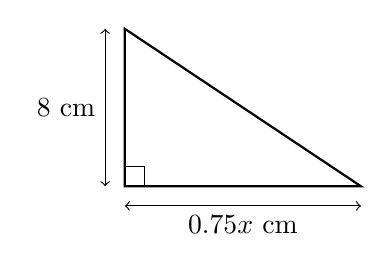
\begin{tikzpicture}[scale=0.5]
  \draw[thick] (0,0) -- (6,0) -- (0,4) -- cycle;
  \draw[<->] (0,-0.5) -- (6,-0.5);
  \node[below] at (3,-0.5) {$0.75x$ cm};
  \draw[<->] (-0.5,0) -- (-0.5,4);
  \node[left] at (-0.5,2) {$8$ cm};
  % right angle mark
  \draw (0,0.5) -- (0.5,0.5) -- (0.5,0);
\end{tikzpicture}
\end{center}
\end{questionText}
\correctAnswer{$x = 8$}
\explanation{Area $= \frac{1}{2} \times 0.75x \times 8 = 3x = 24$. Divide by $3$: $x = 8$. Check: $\frac{1}{2}(0.75 \times 8)(8) = \frac{1}{2}(6)(8) = 24$ \checkmark.}
\end{practiceQuestion}
